% Created 2017-10-16 Mon 22:09
% Intended LaTeX compiler: pdflatex
\documentclass[11pt]{article}
\usepackage[utf8]{inputenc}
\usepackage{lmodern}
\usepackage[T1]{fontenc}
\usepackage{fixltx2e}
\usepackage{graphicx}
\usepackage{longtable}
\usepackage{float}
\usepackage{wrapfig}
\usepackage{rotating}
\usepackage[normalem]{ulem}
\usepackage{amsmath}
\usepackage{textcomp}
\usepackage{marvosym}
\usepackage{wasysym}
\usepackage{amssymb}
\usepackage{amsmath}
\usepackage[version=3]{mhchem}
\usepackage[numbers,super,sort&compress]{natbib}
\usepackage{natmove}
\usepackage{url}
\usepackage{minted}
\usepackage{underscore}
\usepackage[linktocpage,pdfstartview=FitH,colorlinks,
linkcolor=blue,anchorcolor=blue,
citecolor=blue,filecolor=blue,menucolor=blue,urlcolor=blue]{hyperref}
\usepackage{attachfile}
\usepackage[left=1in, right=1in, top=1in, bottom=1in, nohead]{geometry}
\geometry{margin=1.0in}
\usepackage{hyperref}
\usepackage{amsmath}
\usepackage{graphicx}
\usepackage{epstopdf}
\usepackage{fancyhdr}
\pagestyle{fancy}
\fancyhf{}
\usepackage[labelfont=bf]{caption}
\usepackage{setspace}
\setlength{\headheight}{10.2pt}
\setlength{\headsep}{20pt}
\renewcommand{\headrulewidth}{0.5pt}
\renewcommand{\footrulewidth}{0.5pt}
\lfoot{\today}
\cfoot{\copyright\ 2017 W.\ F.\ Schneider}
\rfoot{\thepage}
\chead{\bf{Advanced Chemical Engineering Thermodynamics (CBE 60553)\vspace{12pt}}}
\lhead{\bf{Homework 5}}
\rhead{\bf{Due October 23, 2017}}
\usepackage{titlesec}
\titlespacing*{\section}
{0pt}{0.6\baselineskip}{0.2\baselineskip}
\title{University of Notre Dame\\Advanced Chemical Engineering Thermodynamics\\(CBE 60553)}
\author{Prof. William F.\ Schneider}
\usepackage{siunitx}
\usepackage[version=3]{mhchem}
\def\dbar{{\mathchar'26\mkern-12mu d}}
\setcounter{secnumdepth}{3}
\author{William F. Schneider}
\date{\today}
\title{CBE 60553 Homework}
\begin{document}

\begin{OPTIONS}
\end{OPTIONS}

\noindent \textbf{Solve each problem on separate sheets of paper, and clearly indicate the problem number and your name on each.  Carefully and neatly document your answers.  You may use a mathematical solver like Matlab or Mathematica. Use plotting software for all plots.}

\section{Just a little unstable}
\label{sec:org5d4dcbe}
The energy minimum/entropy maximum principle places bounds on the stability of fundamental equations.  What are the limits of stability with respect to \(T\) and \(v\) of the following Helmholtz fundamental equations?

\begin{enumerate}
\item A monatomic ideal gas:

\begin{equation*}
 a_\text{ig} = \left \{ - RT \ln (v) -1.5 R T \ln (R T) \right\} +\left \{ RT \right \}
\end{equation*}

\item A monatomic van der Waals gas:

\begin{equation*}
  a_\text{vdW} = \left \{ - RT \ln (v-b) -1.5 R T \ln (R T) \right\} +\left \{ RT -a/v
  \right \}
  \end{equation*}
\end{enumerate}

\section{What passes for a law these days\ldots{}.}
\label{sec:orgbf90451}
The van der Waals equation obeys
  the law of corresponding states, so all van der Waals fluids exhibit the same
  vapor-liquid phase equilibrium when presented in reduced variables.

\begin{enumerate}
\item Use the following relationship to derive an expression for the van der Waals
equation in terms of the reduced variable \(v_R = v/v_c\), \(T_R = T/T_c\), and
\(P_R = P/P_c\).
\end{enumerate}

\begin{equation*}
  \left ( \frac{\partial P}{\partial v} \right )_{T=T_c} = \left (
    \frac{\partial^2 P}{\partial v^2} \right )_{T=T_c} = 0
\end{equation*}

\begin{enumerate}
\item Plot the spinodal curve of a van der Waals fluid on a \(P_R, v_R\) diagram.
\end{enumerate}

\section{The two phases of van der Waals}
\label{sec:orga764ce5}
Binodal curves are much trickier to find because they are determined by the equality of the three intensive variables rather than just by the curvature of the free energy.  The ``equal area construction'' is a common numerical approach to finding the binodal points.

\begin{enumerate}
\item Use an equal area construction to compute the reduced saturation pressure and
reduced vapor and liquid volumes at \(T_r = 0.8, 0.85, 0.90, 0.95, 1\).  You will want
to use a numerical solver.

\item Plot the points on the same \(P_R, v_R\) diagram as the spinodal above.

\item (Bonus!) Find the latent entropy and latent enthalpy at  \(T_r = 0.8, 0.85, 0.90, 0.95, 1\), using the fact that:
\begin{equation*}
  \Delta s = \int_{v_l}^{v_g} \left ( \frac{\partial s}{\partial v} \right )_T dv
\end{equation*}
Comment on any trend you find. \textit{Hint:} You'll want to apply a Maxwell relation and a cyclic permutation to the partial derivative before evaluating.

\item (Bonus!) The van der Waals constants of \ce{H2O} are \(a = 0.5609~\text{Pa
      m}^6\text{mol}^{-2}\) and \(b = 30.49\times10^{-6}~\text{m}^3\text{mol}^{-1}\).  Use
your results to estimate \(\Delta H^\text{vap}\) of \ce{H2O} at \SI{1}{atm}.  How does the result compare to the experimental value of \SI{40.64}{kJ/mol}?
\end{enumerate}
\section{Steam at the top of the mountain}
\label{sec:orgb1031ea}
The Clapeyron equation, and its cousin Clausius-Clapeyron, relate observable
  pressure and temperature at a phase boundary to the underlying latent
  quantities.
\begin{enumerate}
\item Determine the value of \(dT/dP\) for water at its normal boiling point (\SI{1}{atm})
of \SI{373.1}{K} given that \(\Delta
   H^\text{vap}(373.1~\text{K})=\SI{40.65}{kJ/mol}\) and the densities of liquid
and vapor are 0.9584 and \SI{0.6010e-3}{\gram\per\milli\liter}, respectively.
Estimate the boiling point of water at \SI{2}{atm}.

\item A liquid boils at \SI{95}{\celsius} at the top of a hill and at \SI{105}{\celsius} at the
bottom.  It's latent heat of vaporization is \SI{1000.}{cal\per\mole}.  What is the height
of the hill?  \emph{Hint:} How does pressure vary with altitude?
\end{enumerate}

\section{Qualitatively in phase}
\label{sec:org68d4d44}
The triple point of oxygen (\ce{O2}) is at \ce{54.3}{K} and \SI{1.14}{torr}; it's
  critical point is at \SI{154.6}{K} and \SI{37828}{torr}; it's normal melting and boiling
  points are \SI{-218.4}{\celsius} and \SI{-182.9}{\celsius}, respectively.
  Sketch the phase diagram of oxygen.  Does it melt under applied pressure in
  the same way that water does?

\section{Quantitatively in phase}
\label{sec:orgbdd7dc2}
Near the triple point the following equations describe the vapor pressure of
    liquid and solid \ce{NH3}:
\begin{equation*}
  \ln P^\text{sat}(l) = 24.38~\text{Pa} - \frac{3063~\text{Pa K}}{T} \quad  \ln P^\text{sat}(s) = 27.92~\text{Pa} - \frac{3754~\text{Pa K}}{T}
\end{equation*}

\begin{enumerate}
\item What are the temperature and pressure at the triple point?
\item What is the latent heat of vaporization?
\item What is the latent heat of sublimation?
\item What is the latent heat of fusion at the triple point?
\end{enumerate}

\section{Are you sure? How sure?}
\label{sec:org3714880}
The two state model allows a simple illustration
  of the principles of the microcanonical ensemble. A closed system is composed of an even
  number of two-state ``atoms,'' each of which can have energy 0 or \(\epsilon\).  The
  system is partitioned into two subsystems of equal size.

\begin{center}
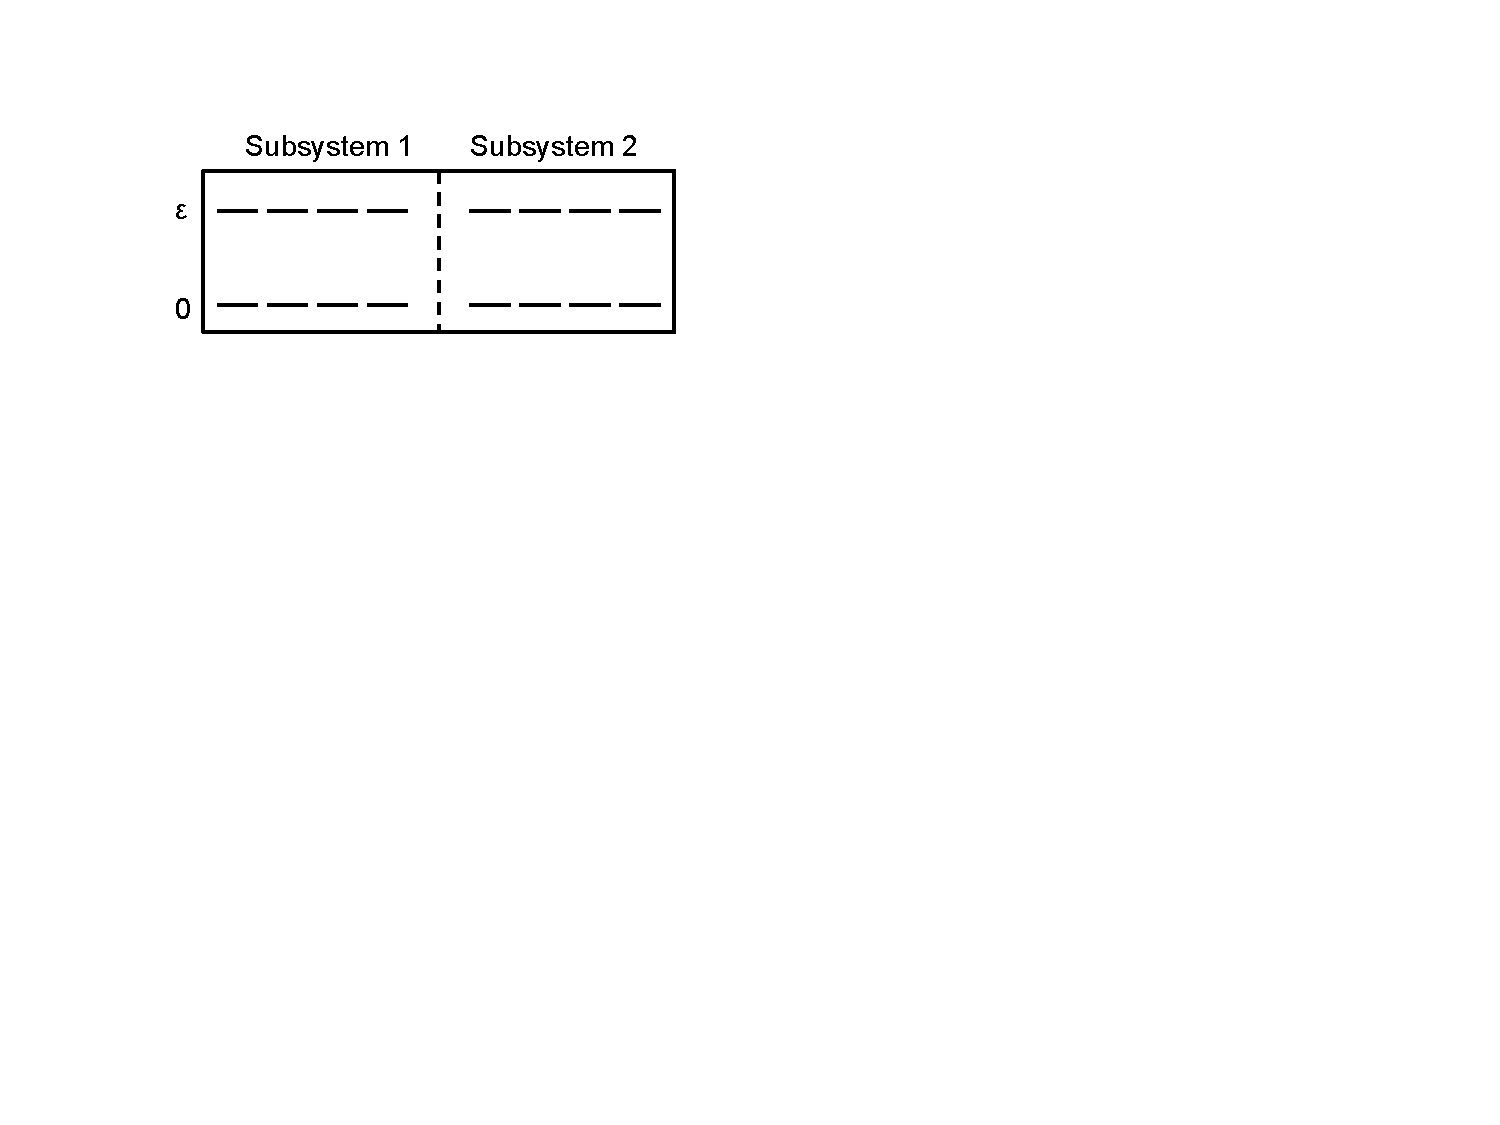
\includegraphics[width=3in]{./figs/Two-state.pdf}
\end{center}

\begin{enumerate}
\item Suppose the system contains 8 atoms as in the figure above, and the total energy of
the system is \(U = 4\epsilon\).  Determine the possible energies \(U_1\) of subsystem 1 and
their relative probabilities.
\item What fundamental assumption did you make to assess the probabilities?

\item The probability distribution you just calculated is called \emph{binomial}
(specifically, binomial with individual probability \(p=1/2\)).  As the sizes of
the subsystems \(N_i\) and the total energy \(U\) grow proportionately, the
probability distribution on \(U_1\) becomes approximately \emph{Gaussian} with mean
\((1/2) N_1\epsilon\) and variance \(\sigma^2 = N_1\epsilon^2\).

\begin{enumerate}
\item Calculate the ratio of the probability that \(U_1=0.51 U\) to \(U_1=0.5 U\) for \(N_1 = 100\).
\item Calculate the ratio of the probability that \(U_1=0.51 U\) to \(U_1=0.5 U\) for \(N_1 = 10^6\).
\item Calculate the ratio of the probability that \(U_1=0.51 U\) to \(U_1=0.5 U\) for \(N_1 = 10^{20}\).
\end{enumerate}

\item What do you think? As \(N_1\) gets really big, what wil \(U_1\) be?  How certain are you?
\end{enumerate}
\end{document}